\chapter{Traversing Potential Energy Surfaces}
\label{chap:pes}

This chapter introduces the idea of potential energy surfaces (PESes) and discusses their creation, interesting features and exploration.
\expand

\section{The Schr\"odinger Equation}
\label{sec:schrodinger}

A central theme in atomic simulations is the solution of the Schr\"odinger equation~\cite{schrodinger-equation-1926}, which is the quantum analogue of Newton's equations of motion~\cite{newton-latin}, governing the motion of the electrons and nuclei, as well as any other observables.
For a non-relativistic system of $N = N_e + N_n$ particles ($N_e$ electrons and $N_n$ nuclei), the time independant Schr\"odinger equation \tred{(Why not the time dependant one?)},
\beq{schrodinger-basic}
 \widehat{H}\Psi = E\Psi,
\eeq
must be solved in order to calculate the total energy of the system, $E$, and the wave function, $\Psi \equiv \Psi(\vr_1, \vr_2, \ldots, \vr_{N_e}, \vR_1, \vR_2, \ldots, \vR_{N_n})$, which depends on the spatial coordinates, $\vr_i$, of each electron and, $\vR_i$, each nuclei, using the total energy operator (more commonly referred to as the Hamiltonian),
\beq{hamiltonian}
\widehat{H} = \sum_i^{N}\widehat{T}_i  + \widehat{V}.
\eeq
Similar to classical systems the Hamiltonian encompasses both kinetic, $\widehat{T}_i = -\nabla_i^2/2$, \footnote{In atomic units} and potential, $\widehat{V} = V(\vR, \vr)$, effects, represented in the traditional R-basis, which will be used exclusively in this thesis.
Though it may look innocent, solving the Schr\"odinger equation, which is a second order partial derivative problem, is a daunting task and in most cases significant approximations must be made.
Efforts to solve the Schr\"odinger equation are discussed below in \fref{sec:methods-qm}.

% ------------------------------------------------------------------
\section{The Born-Oppenheimer Approximation}
\label{sec:born-oppenheimer}
In order to simplify --- and in many cases, make possible --- quantum calculations of large atomic systems, the difference in weight of the electrons and the nuclei\footnote{\mytilde 4 orders of magnitude for hydrogen and more for the heavier elements.} is exploited by performing the calculations in two steps.
First, while the nuclei are kept motionless by excluding their kinetic operator from the Hamiltonian (\fref{eq:hamiltonian}), the electronic wavefunction and energy are determined followed by a calculation for the motion of the nuclei.
The assumption is, essentially, that for any motion of the nuclei, the electrons will move instantly and relax to their ground state to accommodate.
This is commonly known as the Born-Oppenheimer approximation.\cite{born-oppenheimer-1927}

\figmiss{Example PES, high priority}

This decoupling allows for a mapping of the potential energy as a function of the nuclear coordinates (commonly referred to as the potential energy surface or PES), as opposed to the continuum of PESes which exist should the motion of the nuclei and electrons be determined simultaneously.
PESes are, generally, not known \textit{a priori} and much effort is spent on traversing them to discover interesting features, such as minima, which represent stable atomic structures, or, as we shall see below, reaction pathways.

%\url{http://www.search.com/reference/Born-Oppenheimer_approximation}
%Should be bad for metallic systems but has proved useful nevertheless. \footnote{see \url{http://www.nature.com/nmat/journal/v6/n3/pdf/nmat1846.pdf}}
%\url{http://www.jhu.edu/~chem/yarkony/research.html} specializes in non-BOA calculations.

All the work carried out in this thesis employs this approximation.

\section{Quantum Calculations}
\label{sec:methods-qm}

% Add a footnote about the spin density DFT (see Kieron's stuff for a reference)
% Also footnote on degeneracy

With increased computing power and, in particular, advances in parallel algoritms, it is now possible to calculate a range of physical properties for materials at the atomic level without the use of any experimental parameters.
Such \textit{ab initio} methods are generally attempts at solving or approximating the Schr\"odinger equation (\fref{sec:schrodinger}) for the ground state\footnote{Non ground state calculations are not considered in this thesis.}.
Multiple strategies exist --- choosing one generally involves considering the trade-off between accuracy and computational effort --- but the main one used in this thesis is the Density Functional Theory, where the many-electron problem is \emph{exactly} divided into multiple one-electron problems.
%\expand?

\subsection{The Electronic Structure Problem}
Solving the Schr\"odinger equation (\fref{sec:schrodinger}) is not a menial task, as it is a second order partial derivative equation in multiple dimensions and can only be solved exactly for very small systems.
Due to the high dimensionality of the wavefunction, simply storing it for a medium-to-large system is physically impossible.\footnote{Consider a system of only $16$ electrons (e.g. an oxygen molecule), sampled on a grid of $10$ points in each direction. Since each electron has 3 degrees of freedom the number of gridpoints will be $10^{16\times3} = 10^{48}$. Compared with the estimated amount of atoms in/on the Earth, $\mytilde10^{50}$, the amount of gridpoints is impossible to store, even for a modest system. This problem is commonly referred to as the exponential wall~\cite{kohn-1999}}

The Born-Oppenheimer approximation (\fref{sec:born-oppenheimer}) allows the separation of the Hamiltonian to an electronic part and a nuclear part.
Thus, the positions of the nuclei, $\vR_I$, only enter the calculations as parameters.
A full quantum treatment will not be discussed here as the goal is to build a PES.

A non-relativistic system of $N_e$ electrons (and $N_n$ nuclei) is described by the time independent Schr\"odinger equation~\cite{schrodinger-equation-1926}
\beq{schrodinger-basic-again}
 \widehat{H}\Psi = E\Psi,
\eeq
where $\Psi \equiv \Psi(\vr_1, \vr_2, \ldots ,\vr_{N_e})$ is the wave function, depending on the spatial coordinates, $\vr_i$, of each electron, $E$ is the electronic energy of the system and $\widehat{H}$ is the Hamiltonian,
\beq{hamiltonian-full}
\widehat{H} = -\frac{1}{2} \sum_i^{N_e} \nabla^2_i + \sum_i^{N_e} \sum_{j>i}^{N_e} \frac{1}{\left| \vr_i - \vr_j \right|} + \sum_i^{N_e} \sum_I^{N_n} \frac{1}{\left| \vr_i - \vR_I \right|} + \widehat{V}_\text{env},
\eeq
which consists of 4 terms.
First there is the kinetic energy of the electrons, $\widehat{T}_\text{e} = -2^{-1}\sum_i^{N_e}\nabla_i^2$,
then the electron-electron interaction, $\widehat{U}_\text{ee} = \sum_i^{N_e}\sum_{j>i}^{N_e}(\left| \vr_i - \vr_j \right|)^{-1}$,
followed by the electron-nuclei interaction, $\sum_i^{N_e}\sum_I^{N_n}(\left| \vr_i - \vR_I \right|)^{-1}$,
and finally any further environmental influence (e.g. an applied electric field) is represented by a single term, $\widehat{V}_\text{env}$.
The last two terms are often bundled into a single external term,
\beq{hamiltonian-external}
V_\text{ext} = \sum_i^{N_e} \sum_I^{N_n} \frac{1}{\left| \vr_i - \vR_I \right|} + V_\text{env},
\eeq
since these are system dependant, while $\widehat{T}_\text{e}$ and $\widehat{U}_\text{ee}$ can be considered universal.

\subsection{Density Functional Theory}
\label{sec:methods-dft}
One of the most popular and common techniques for solving the electronic structure problem is the Density Functional Theory (DFT) which can exactly (in theory) solve the Schr\"odinger equation.
However, in practice, approximations must be made for all but the most simple systems.
Nevertheless, DFT has produced many interesting and good results and is now a well established formalism that is continually being reviewed and improved.
Furthermore, the \textit{ab initio} nature of DFT makes it a great companion to experimental research, not only for comparison and prediction of interesting materials but also to assist and expand upon data analysis.

The success of DFT yielded one of its founders, Walter Kohn, one half of the Nobel Prize in chemistry in 1998, for the development of the density functional theory~\cite{kohn-1999} along with John Pople for his development of computational methods in quantum chemistry~\cite{pople-1999}.

\subsubsection{The Hohenberg-Kohn Theorems}
The earliest mention of a DFT type method were made by Thomas~\cite{thomas-1927} and Fermi~\cite{fermi-1927} but the heart of DFT lies in the Hohnberg-Kohn theorem, which reformulates the electronic structure problem to depend on the $3$ dimensional, ground state, electron density, $\rho_0(\vr)$, instead of the $3N$ dimensional wavefunction, $\Psi(\vr_1, \vr_2, \ldots, \vr_N)$.
According to the first Hohenberg-Kohn theorem~\cite{hohenberg-kohn-1964}, any external term, $V_\text{ext}$, in \fref{eq:hamiltonian-full} yields a different electron density from any non-identical $V'_\text{ext}$ up to trivial additive constant, for the ground state.
In other words: there is a one-to-one correspondence between the wavefunction and the electron density of the ground state and all observables that depend on the wavefunction can, thus, be extracted from the ground state density.
This allows a re-formulation of the Schr\"odinger equation, with the energy as a functional of the electron density, 
\beq{reformulated-schrodinger-equation}
E[\rho_0] = \bra \Psi[\rho_0] | \widehat{H} | \Psi[\rho_0] \ket.
\eeq

Furthermore, the second Hohenberg-Kohn theorem~\cite{hohenberg-kohn-1964} adds a variational~\cite{variational-rayleigh-1870, variational-ritz-1909} way to discover the true ground state density and ground state energy,
\beq{variational-density}
E_0 = \min_\rho E[\rho].
\eeq

This work alone is still missing key elements in order to efficiently solve for the wavefunction and energy, namely the wavefunction to density mapping is not known.

\subsubsection{The Kohn-Sham Equations}
Counter-intuatively re-introducing wave functions was the solution proposed by Walter Kohn and Lui Jeu Sham in 1965~\cite{kohn-sham-1965}.
Inspired by Hartree's work nearly four decades earlier~\cite{hartree-1928}, multiple non-interacting single particle wave functions, $\phi_i(\vr_i)$, took the place of the many-body wave function (or electron density), such that
\beq{kohn-sham-density}
 \rho(\vr) = \sum_{i=1}^{N_e} \left| \phi_i(\vr_i) \right|^2,
\eeq
where each electron would be subject to an effective potential, $v(\vr)$, due to all the particles in the system (including itself, the nuclei and any external factors).
Solving for $\phi_i$ and $\epsilon_i$ (the Kohn-Sham energies) using multiple Schr\"odinger type equations (commonly referred to as the Kohn-Sham equations),
\beq{kohn-sham-equations}
 \left\{-\frac{1}{2} \nabla ^2 + v(\vr) \right\} \phi_i(\vr_i) = \epsilon_i \phi_i(\vr_i),
\eeq
can be done iteratively in a variational manner, from an initial guess for the electron density.

Constructing the effective potential becomes the main problem here, since an exact $v(\vr)$ yields an exact solution to the whole electronic structure problem.
The external potential, $\widehat{V}_\text{ext}$, from \fref{eq:hamiltonian-external} enters unchanged as it contains only static information.
Conversely, the electron-electron interaction, $\widehat{U}_\text{ee}$, enters in a changed form.
In fact, it is introduced as two terms, one for interaction with the electron density as a whole, commonly referred to as the hartree potential ($v_\text{H}(\vr)$) and a second one for many-electron and Pauli-exclusion effects, %self-interaction effects, 
$v_\text{XC}(\vr)$, the so-called exchange-correlation potential,
\beq{effective-potential}
v(\vr) = V_\text{ext}(\vr) + v_\text{H}(\vr) + v_\text{XC}(\vr).
\eeq
The hartree potential is an integral over the electron density,
\beq{hartree-potential}
v_\text{H}(\vr) = \int \frac{\rho(\vr')}{\left| \vr - \vr' \right|}d^3\vr',
\eeq
and the exchange-correlation potential is of the form,
\beq{exchange-correlation-potential}
v_\text{XC}(\vr) = \frac{\partial E_{XC}[\rho(\vr)]}{\partial \rho(\vr)}.
\eeq

Thus far the formalism is exact, however, all the difficult parts, $E_\text{XC}[\rho(\vr)]$, have yet to be discussed.

\subsubsection{The Exchange-Correlation Functional}
The Kohn-Sham equations are in principle exact, however, the exchange-correlation functional, $E_\text{XC}[\rho(\vr)]$, is generally not known and has to be approximated.
The accuracy of this approximation is a major factor in determining the accuracy of DFT as a whole.
A detailed discussion of Exchange-Correlation functionals is material enough for a whole chapter, thus only the basic approximation will be discussed here.

The Local Density Approximation (LDA)~\cite{kohn-sham-1965} treats exchange-correlation as if it were a homogeneous electron gas.
The exchange part is known exactly,
\beq{exchange-lda}
E_\text{X}^\text{LDA}[\rho(\vr)] = - \frac{3}{4} \sqrt[3]{\frac{3}{\pi}} \int \sqrt[3]{\rho^4(\vr)}.
\eeq
The correlation part, however, is not known but has been tabulated using accurate Quantum Monte-Carlo simulations.~\cite{correlation-1980}

Multiple exchange-correlation functionals exist, each with different strong suits, some fitted to empirical data\footnote{putting into question their \textit{ab initio} nature.}~\cite{blyp-1993}, while others are hybrids of previous functionals~\citemiss.
Those mainly used in this thesis are of the generalised gradient approximation (GGA) variety~\cite{gga-original-1986, gga-1996, pw91}, similiar to LDA but the gradient is also taken into account.

%\beq{xc-lda}
%E_\text{XC}^\text{LDA}[\rho(\vr)] = \int \epsilon_\text{XC}^\text{hom.}[\rho(\vr)]\rho(\vr)d^3\vr,
%\eeq
%where $\epsilon_\text{XC}^\text{hom.} = \epsilon_\text{X}^\text{hom.} + \epsilon_\text{C}^\text{hom.}$ is the exchagne-correlation density.
%$\epsilon_\text{X}^\text{hom.}$ 



%\tred{I've removed the Implementation (DACAPO) section. Including it and a PAW section would be nice. Also included a list of stuff DFT is good/bad for would make sense. High priority}
%The approximations used in our work are based on the so-called Generalized Gradient Approach (GGA). The GGA uses the the exchange-correlation energy of a homogeneous electron gas at point $\vect{r}$ like the Local Density Approximation (LDA) \cite{kohn1965} but also uses the gradient of the density to account for inhomogeneity. This, however, is not a good choice by itself so a reduced density gradient, $s(\vect{r})$, is used, as suggested by Langreth and Perdew \cite{langreth1977}. The exchange-correlation functional then becomes
%\begin{equation}
%  E_{XC}^{GGA}[\rho] = \int d^3r\, \epsilon_{XC}^{GGA}(\rho(\vect{r}), s(\vect{r}))\rho(\vect{r})
%\end{equation}
%with
%\begin{equation}
%\label{eq:GGAreducedDensityGradient}
% s(\vect{r}) = \frac{\left|\nabla \rho(\vect{r})\right|}{2\sqrt[3]{3\pi^2\rho(\vect{r})} \rho(\vect{r})}.
%\end{equation}

%\subsection{Implementation of DFT}
%\label{sec:methods-dft-implemetnation}
%
%\subsubsection{The Plane Wave Basis Set}
%In implementing DFT calculations, the Kohn-Sham wavefunctions are expanded in a particular basis set. In our work plane waves are used under periodic boundary conditions in accordance with Bloch's theorem,
%\begin{equation}
%\label{eq:blochsTherom}
% \psi_\vect{k}^{m}(\vect{r}) = \sum_\vect{G}c_{\vect{k} + \vect{G}}^m\, e^{i(\vect{k}+\vect{G})\cdot\vect{r}}
%\end{equation}
%where $\vect{G}$ are the reciprocal lattice vectors. %[what are $c_{\vect{k} + \vect{G}}^m$?]. 
%For an exact solution, an infinite number of plane waves is needed. Fortunately the plane waves at the lower end of the kinetic energy range are the most important, so the number of plane waves can be reduced by defining a cutoff, $G_{cut}$, where the solution becomes good enough:
%\begin{equation}
% \left( \frac{\hbar^2}{2m} \right) \left| \vect{k} + \vect{G}_{cut} \right|^2 \le E_\mathrm{cut}.
%\end{equation}
%This leads to one of the main advantages of plane waves. By increasing the cutoff the accuracy of the calculation can be systematically increased. 
%
%A disadvantage of plane waves is their inefficiency to deal with high curvature regions, such as the atomic core. To overcome this pseudopotentials can be used. In the core, pseudopotentials are an average of the potential due to the core electrons and the nucleus felt by the valence electrons inside a given sphere but outside the sphere the pseudopotential becomes identical to the all-electron potential. The plane-wave cutoff can be lowered even further when using pseudopotentials while generally giving results of good accuracy, especially the so-called ultrasoft pseudopotential with non-local components \cite{vanderbilt1990}.
%
%\subsection{Known Problems of DFT}
%\bit
%\item Band Gaps in semi conductors
%\item Dispersion (van Der Waals)
%\item etc.
%\eit
%
%\placeholder

\section{Analytical Potential Energy Surfaces}
\label{sec:potentials}
For very large systems or when timing is a factor, it is possible to employ classical potential functions for calculating the potential energy and gradient.
Such potential functions are tailor made for a given bond and generally give poor physical insight when used on a different system.

Most common are pair-potentials\footnote{Many-body potentials are also possible (see for example~\cite{stillinger-weber-potential})}, where each atom in the system feels an interaction with every other atom up to a cut-off radius, and this interaction can be tuned by empirical parameters.
Such potentials are very helpful during the development of methods and two such were extensively used for testing the novel method presented in \fref{chap:erm} and paper \ref{pap:second-order}.~\cite{eam-1983, eam-1986, emt-1987, emt-1996}
Furthermore, if tuning the parameters of the potential well enough is possible, the potential can be used to perform calculations that are infeasible for quantum methods, such as long term molecular dynamics of large systems.~\citemiss

\subsubsection{Embedded Atom Model}
The Embedded Atom Model (EAM)~\cite{eam-1983} operates under the principle that an atom's energy is a functional of the system's electron density.
Its basic formula for the energy of atom $i$ is
\beq{eam}
E_i = F_\alpha \left( \sum_{i \not= j} \rho_\beta(\left| \vR_i - \vR_j \right|)\right) + \frac{1}{2} \sum_{i \not= j}   \phi_{\alpha\beta}(\left| \vR_i - \vR_j \right|),
\eeq
where $\phi_{\alpha\beta}$ is a short-range pairwise-potential function, $\rho_\beta$ is the contribution to the electron charge density from atom $j$ of type $\beta$ at $\vR_i$ and $F_\alpha$ is an embedding function that represents the energy required to place atom $i$ of type $\alpha$ into the electron cloud.

EAM has been parametrised very well, e.g. for \ce{Al} surfaces using DFT data~\cite{eam-1986} and used successfully in studies of the self-diffusional mechanisms on the \ce{Al}(100) surface~\cite{dimer-original-1999}

Extensive use was made of potential functions in this thesis.
Simple and quick test cases served to produce PESes that could be visualised in two dimensions, while still retaining the properties of truly multidimensional systems in \fref{chap:erm}.
While more extensive tests were carried out in \fref{chap:al} on systems that are known to be described well with analytical PESes.


\section{Force}
\label{sec:force}
Since the PES, $E(\vR)$, is, generally, not known \textit{a priori}, traversing it is difficult without a guide.
Such a guide exists in the form of the gradient, $\nabla E(\vR)$, in which information about the increase/decrease of the function (here: PES) is encoded.
The gradient points towards the direction of greatest increase, however, in atomic simulations such areas are, commonly, of little interest.
Most of the time, systems are at, or near, stable structures, which are represented by minima on the PES.
Defining a force that, similarly to real world forces, points the system towards areas of lowest potential energy, is straight forwards as the negative gradient,
\beq{force-general}
\vF(\vR) = -\nabla E(\vR).
\eeq

The gradient is not directly available from DFT calculations, as for other non-analytical PESes.
Fortunatelly, for variational calculations, such as DFT, a force theorem has been developed, stating that $\partial E / \partial\lamda$ can be evaluated for for a continous parameter $\lambda$ on which the wavefunction, $\Psi(\lambda)$, depends implictily,
\beq{hellmann-feynman-forces-full}
\frac{\partial E}{\partial \lambda} = 
\bra \frac{\partial \Psi}{\partial \lambda} | \widehat{H} | \Psi \ket +
\bra \Psi | \frac{\partial \widehat{H}}{\partial \lambda} | \Psi \ket +
\bra \Psi | \widehat{H} | \frac{\partial \Psi}{\partial \lambda} \ket.
\eeq
Utilizing the orthogoanlity of the wave function, the first and last terms are zero, 
\beq{hellmann-feynman-forces-final}
\frac{\partial E}{\partial \lambda} = \bra \Psi | \frac{\partial \widehat{H}}{\partial \lambda} | \Psi \ket.
\eeq
Once the electronic wave function has been constructed, which is the most time consuming part, the gradient can be calculated.
For DFT, and any other Born-Oppenheimer calculation, $\lambda$ can be the nuclear coordinates.
%\beq{dft-nuclear-forces}
%\vF_\lambda = \frac{\partial E}{\partial \vR_\lambda} = \bra \Psi | \frac{\partial \widehat{H}}{\partial \vR_\lambda} | \Psi \ket = 
%\eeq

The theorem has been proved independantly by multiple authors~\cite{forces-pauli-1933, forces-guttinger-1932} but is generally attributed to Richard Feynman\cite{forces-feynman-1939} and Hans Hellmann~\cite{forces-hellmann-1937}, as the Hellmann-Feynmann Theorem.

\section{Locating Minima}
\label{sec:minima}
Searching for minima\footnote{or equivalently maxima but due to the context of atomic simulations the discussion will be on minima.} is an important subject as they represent stable structures on PESes.
Using the available local information, the energy and the force, it is possible to follow the force with an appropriate step size until the gradient is zero, at which time a stationary point has been reached.
Generally this point will be a minimum but classifying non-minima will be discussed below.

Multiple techniques exist for performing these minimisations\footnote{Also often referred to as optimisations} in as few iterations as possible.
Some are as simple as adjusting the step size to simulate velocity, while others detect changes in this fictional velocity and adjust accordingly~\cite{cg-original-1952, fire}.
Still other methods build up information about the curvature and assume a quadratic environment~\cite{lbfgs}.

All these methods have a common theme of solving Newton's equations of motion with some type of fictional friction in order to reduce the kinetic and total energy of the system to bring it to a potential energy minimum.

\section{The Hessian Matrix}
\label{sec:hessian}

For a real function $f$ of $n$ variables, $\vect{x} = (x_1, x_2, \ldots, x_n)$,
there exists an $n\times n$ matrix, $\text{H}$, which contains all the second partial derivatives,
\beq{hessian-matrix}
\text{H} =
\begin{bmatrix}
\vspace{0.5em} % To create a bit of space AFTER the first line.
\frac{\partial^2f}{\partial x_1^2} &
\frac{\partial^2f}{\partial x_1 \partial x_2} &
\cdots &
\frac{\partial^2f}{\partial x_1 \partial x_n} \\

\frac{\partial^2f}{\partial x_2 \partial x_1} &
\frac{\partial^2f}{\partial x_2^2} & 
\cdots &
\frac{\partial^2f}{\partial x_2 \partial x_n} \\

\vdots & \vdots & \ddots & \vdots \\

\frac{\partial^2f}{\partial x_n \partial x_1} &
\frac{\partial^2f}{\partial x_n \partial x_2} &
\cdots &
\frac{\partial^2f}{\partial x_n^2} &
\end{bmatrix}.
\eeq
The second derivative of a function represents, in particular, information about its local curvature, or how rapidly the first derivative changes.
Classification of stationary points (and implicitly critical points) relies on the eigenvalues of $\text{H}$, $\lambda_i$,
\bit
\item Minimum if all $\lambda_i > 0$
\item Maximum if all $\lambda_i < 0$
\item Saddle Point if some but not all $\lambda_i < 0$
\item Otherwise higher order derivatives are needed for classification
\eit

$\text{H}$ is named after the German mathematician Ludwig Otto Hesse and is commonly referred to as the Hessian matrix, or Hessian for short~\cite{hessian}.

In the context of atomic simulations, $n$ is generally 3 times the number of atoms in the system, as each one has 3 independent degrees of freedom and the function in question is often the potential energy of the system.
In most modern software packages both the potential energy and force are readily available while the second order derivatives are, generally, not available without explicit and, often, costly calculations.

\section{Saddle Points}
\label{sec:sps}

%\figmiss{I'd like to have a saddle for horse riding as a comparison here. VERY low priority.}

Saddle points are stationary points, i.e. with zero gradient, on a multidimensional function, $f(\vR)$, that are neither maxima nor minima.

\begin{figure}[h]
  \begin{center}
  \subfigure[2D saddle point][2D saddle point, $f(x=0, y=0) = x^2 - y^2$. A minimum is the $x$ direction and a maximum in the $y$ direction]{
    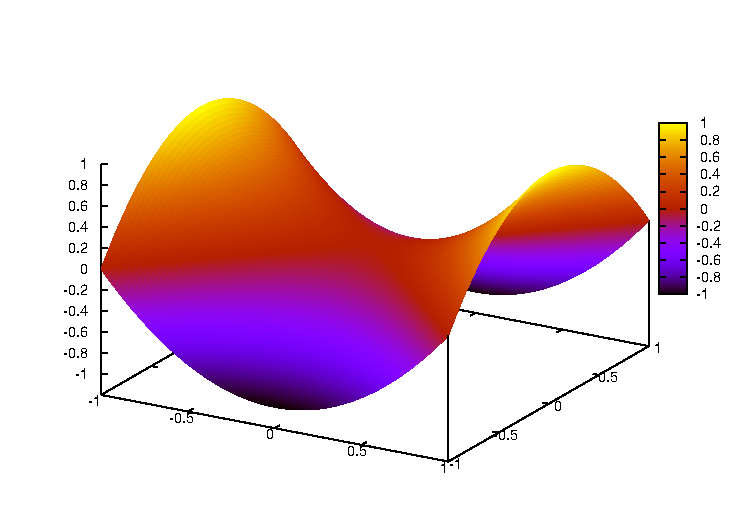
\includegraphics[width=0.6\linewidth]{saddle-point-2d}
    \label{fig:2d-saddle-point}
    }
  \subfigure[1D saddle point][1D saddle point, $f(x=0) = x^3$. Neither a maximum nor a minimum but the gradient is vanishing.]{
    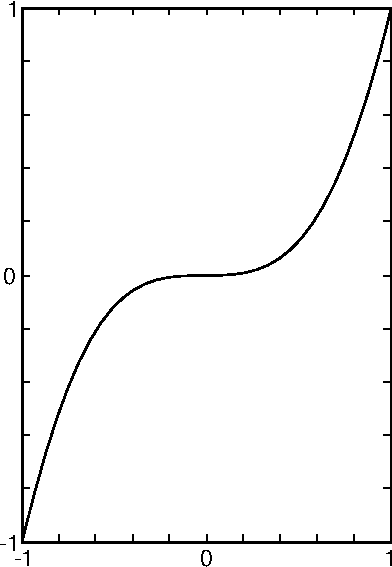
\includegraphics[width=0.26\linewidth]{saddle-point-1d}
    \label{fig:1d-saddle-point}
    }
    \parbox{0.85\linewidth}{
      \caption{Examples of first order saddle points.
      }
      \label{fig:saddle-points}
    }
  \end{center}
\end{figure}

A common view of a saddle (point) can be found in \fref{fig:2d-saddle-point}, as the function $f(x, y) = x^2 - y^2$ which near $(x,y) = (0,0)$ resembles a saddle, used when riding horses, curving upwards in one direction (along the horse) and downwards in the other (perpendicular to the horse).
This image of a saddle point lacks a few elements to tell their whole story but acts as a good general case.
On functions of higher dimensionality than $2$, different orders of saddle points are possible.
The order of the saddle point is decided by the amount of directions that are not at a minimum, or the non-positive eigenvalues of the Hessian.
As such, \fref{fig:2d-saddle-point} shows a first order saddle point on a two dimensional function.
In this thesis, saddle points of order $N$ will be indicated by \sap{N} from here on.

The Hessian at the \sap{} displayed in \fref{fig:2d-saddle-point} has one negative eigenvalue, however, a saddle point with one or more vanishing eigenvalues is also possible, such as the 1D example $f(x = 0) = x^3$, seen in \fref{fig:1d-saddle-point}.

Locating \sap{}s in multiple dimensions is a non-trivial task as only a limited number of steepest decent paths lead to each one while the majority lead to minima.
A number of schemes  for locating \sap{1}s have been suggested (see \cite{sp-mep-review-2002} for a review), out of which two popular ones are discussed in \fref{chap:saddle-point-methods}: The Dimer method and the Nudged Elastic Band method.
Furthermore, an extension to these methods for finding higher order \sap{}s is presented in \fref{chap:erm}.

In the context of atomic simulations, \sap{}s are important in describing reactions and reaction rates.

\section{Steepest Descent Paths}
\label{sec:sdps}
\begin{figure}[h]
  \begin{center}
    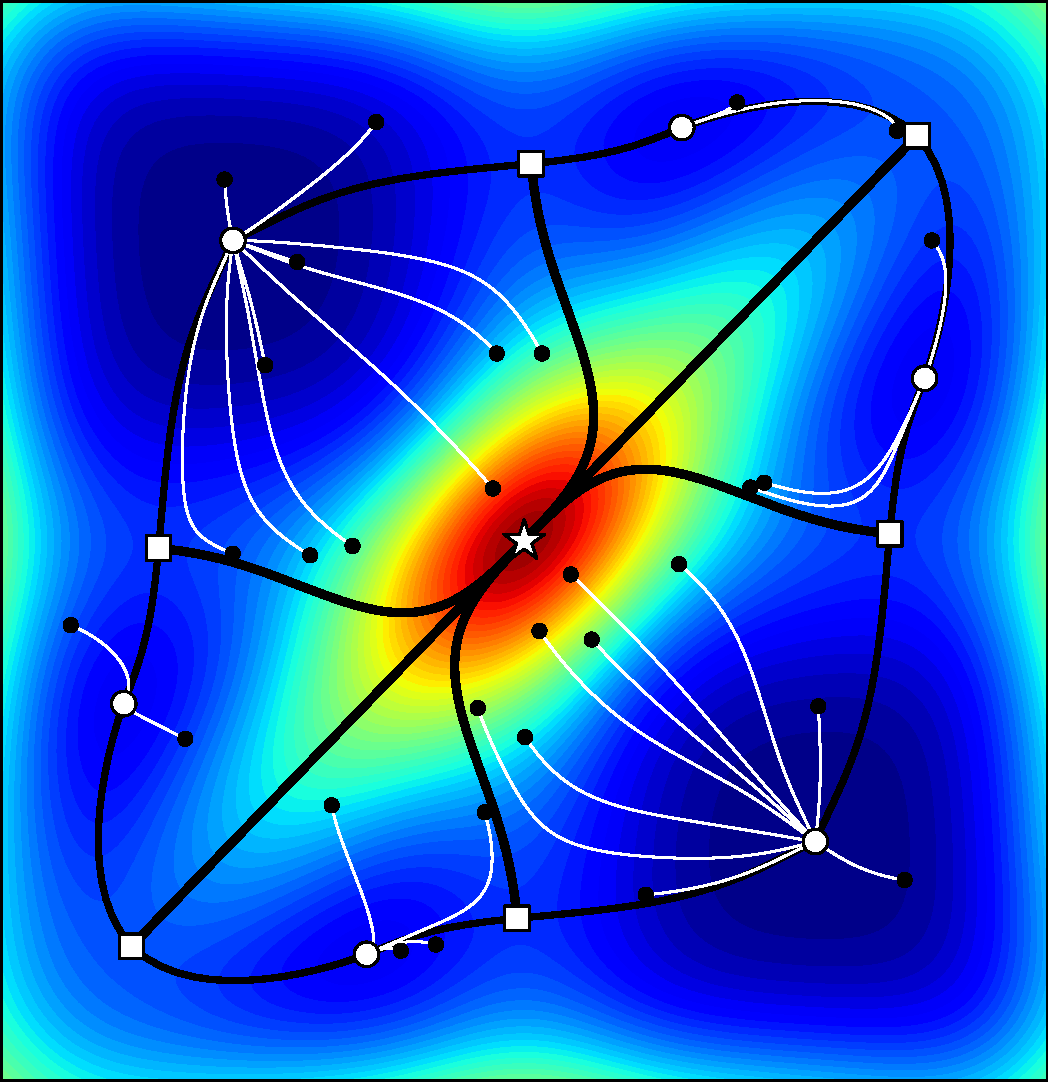
\includegraphics[width=0.6\linewidth]{paths}
    \parbox{0.85\linewidth}{
      \caption{Examples of steepest descent paths.
The white symbols represent stationary points, the circles are minima, the squares are \sap{1}s and the star is a \sap{2}.
The black circles are starting points for random SDPs (the white lines).
The black lines are specific SDPs, the dotted ones are ridges while the solid ones are MEPs.
      }
      \label{fig:paths}
    }
  \end{center}
\end{figure}

Steepest Descent Paths (SDPs) are paths on a multidimensional function, $f$, for which there is no perpendicular gradient component,
\beq{sdp-definition}
\nabla \vect{f} - (\nabla \vect{f} \cdot \uvt)\uvt = \vect{0},
\eeq
where $\uvt$ is the tangent to the path.
They can be created by following the negative gradient until it vanishes.
SDPs can begin anywhere, apart from points with a vanishing gradient, but, generally, end at minima (most common) or \sap{}s.
Two sorts of SDPs are of particular interest for the work presented in this thesis, both of which are discussed below.

\subsubsection{Minimum Energy Paths}
The Minimum Energy Path (MEP) is a collection of two specific SDPs, used in the context of theoretical reaction chemistry and represents a likely reaction path on the PES.
It connects two neighbouring minima through a \sap{1} (and through any intermediate \sap{1}s with a lowest Hessian eigenvalue of zero), where each SDP begins~\cite{neb-polemic-henkelman1}, with an infinitesimal displacement along the path.

\subsubsection{Ridges}
Similar to MEPs, ridges are collections of specific SDPs, but with their starting points at \sap{2}s and their end points in \sap{1}s.
Of course, MEPs do not exist near \sap{2}s, and the analogue ends there as the criterion for a ridge demands a negative eigenvalue in the reduced Hessian, perpendicular to the path.

